\documentclass[10pt]{article}

\usepackage{graphics}
\usepackage{dirtree}
\usepackage{paracol}
\usepackage{epigraph}
\usepackage{enumitem}
\usepackage{xcolor}

\setlength{\textwidth}{17cm}
\setlength{\oddsidemargin}{-1cm}
\setlength{\evensidemargin}{-1cm}
\setlength{\textheight}{26cm}
\setlength{\parindent}{0pt}
\setlength{\parskip}{0.3ex}

\usepackage{fancyhdr}
\usepackage{epsfig}
\usepackage[utf8]{inputenc}
\usepackage[french]{babel}
\usepackage[T1]{fontenc}
%\usepackage{verbatim}
\usepackage{graphics}
\usepackage{amsmath,amsfonts,amssymb}
\usepackage{listings}
\usepackage{thmbox}
\usepackage{comment}

\oddsidemargin=0cm
\evensidemargin=0cm
\textwidth=17cm
\textheight=25cm
\topmargin=0mm
\hoffset=-6mm
\voffset=-25mm
%\headsep=30pt

\newcounter{numpartie}
\newcounter{exo}
\newcommand{\partie}[2]
{
        \refstepcounter{numpartie}
        \setcounter{exo}{0}
        \vspace{3mm}

        %\noindent{\large\bf Partie \Alph{numpartie}~-~#1}\hfill
        \noindent{\large\bf Partie \Alph{numpartie}~ ~#1}\hfill
        %[\;{\it bar\^eme indicatif : #2}\;]\\
        \\

}

\newenvironment{exercice}{\refstepcounter{exo} \vspace*{1em}\begin{thmbox}[S]{{\bf Exercice \arabic{exo}~:}}}{\end{thmbox}}

\newenvironment{solution}{\vspace*{1em}\begin{thmbox}[S]{{\bf Solution~:}}}{\end{thmbox}}

\newcommand{\IGNORE}[1]{}

\def\EnteteUE{
\noindent{\bf Université Grenoble Alpes} \hfill {\bf DLST}

\vspace{-8pt}

\noindent\hrulefill

\vspace{-2pt}

\noindent{\bf UE INF203} \hfill {\bf Année 2017-18}

\vspace*{.5cm}
}

\newcommand{\PiedDePageUE}[1]{
\fancypagestyle{monstyle}
{
\rhead{}
\lfoot{{\bf\small INF203 - 2016/2017}}
\cfoot{\thepage}
\rfoot{{\it #1}}
\renewcommand{\footrulewidth}{0.5pt}
\renewcommand{\headrulewidth}{0.0pt}
}
\pagestyle{monstyle}
}


\newcounter{question}
\newenvironment{question}[1][]{\refstepcounter{question}
   \textbf{[\bf \alph{question}] {\begin{emph}{#1}\end{emph}}}}{~$\blacksquare$~\\}

\newcommand{\unix}[1]{\hspace*{2cm}{\bf \tt #1}}
\newcommand{\fich}[1]{{\bf \em #1}}
\newcommand{\ecran}[1]{{\tt #1}}
\newcommand{\C}[1]{{\tt #1}}
\newcommand{\cmd}[1]{{\bf #1}}
\newcommand{\home}{\~{}}

\newenvironment{exocomp}{\vspace*{1em}\begin{thmbox}[M]{Exercice complémentaire :~}}{\end{thmbox}}


\begin{document}
\thispagestyle{empty}

\definecolor{mygreen}{rgb}{0,0.6,0}
\definecolor{mygray}{rgb}{0.5,0.5,0.5}
\definecolor{mymauve}{rgb}{0.58,0,0.82}

\lstdefinestyle{customc}{
  belowcaptionskip=1\baselineskip,
  breaklines=true,
  frame=L,
  xleftmargin=\parindent,
  language=C,
  showstringspaces=false,
  basicstyle=\footnotesize\ttfamily,
  keywordstyle=\bfseries\color{green!40!black},
  commentstyle=\itshape\color{purple!40!black},
  identifierstyle=\color{blue},
  stringstyle=\color{orange},
}

\lstdefinestyle{none}{
  belowcaptionskip=1\baselineskip,
  breaklines=true,
  frame=L,
  xleftmargin=\parindent,
  language=bash,
  showstringspaces=false,
  basicstyle=\footnotesize\ttfamily,
  keywordstyle=\bfseries\color{black},
  commentstyle=\itshape\color{black},
  identifierstyle=\color{black},
  stringstyle=\color{black},
}

\lstset{tabsize=3, style=customc,literate=
  {á}{{\'a}}1 {é}{{\'e}}1 {í}{{\'i}}1 {ó}{{\'o}}1 {ú}{{\'u}}1
  {Á}{{\'A}}1 {É}{{\'E}}1 {Í}{{\'I}}1 {Ó}{{\'O}}1 {Ú}{{\'U}}1
  {à}{{\`a}}1 {è}{{\`e}}1 {ì}{{\`i}}1 {ò}{{\`o}}1 {ù}{{\`u}}1
  {À}{{\`A}}1 {È}{{\'E}}1 {Ì}{{\`I}}1 {Ò}{{\`O}}1 {Ù}{{\`U}}1
  {ä}{{\"a}}1 {ë}{{\"e}}1 {ï}{{\"i}}1 {ö}{{\"o}}1 {ü}{{\"u}}1
  {Ä}{{\"A}}1 {Ë}{{\"E}}1 {Ï}{{\"I}}1 {Ö}{{\"O}}1 {Ü}{{\"U}}1
  {â}{{\^a}}1 {ê}{{\^e}}1 {î}{{\^i}}1 {ô}{{\^o}}1 {û}{{\^u}}1
  {Â}{{\^A}}1 {Ê}{{\^E}}1 {Î}{{\^I}}1 {Ô}{{\^O}}1 {Û}{{\^U}}1
  {œ}{{\oe}}1 {Œ}{{\OE}}1 {æ}{{\ae}}1 {Æ}{{\AE}}1 {ß}{{\ss}}1
  {ű}{{\H{u}}}1 {Ű}{{\H{U}}}1 {ő}{{\H{o}}}1 {Ő}{{\H{O}}}1
  {ç}{{\c c}}1 {Ç}{{\c C}}1 {ø}{{\o}}1 {å}{{\r a}}1 {Å}{{\r A}}1
  {€}{{\euro}}1 {£}{{\pounds}}1 {«}{{\guillemotleft}}1
  {»}{{\guillemotright}}1 {ñ}{{\~n}}1 {Ñ}{{\~N}}1 {¿}{{?`}}1
}

\EnteteUE

\begin{center}
  {\large {\bf Corrigé TP7}}
\end{center}

\vspace*{0.5cm}

\begin{enumerate}[label=\textbf{[\alph*]}]
  \setlength\itemsep{1em}

\item Par défaut, lorsque l'automate est appelé avec la fonction
  \texttt{init\_par\_defaut}, toutes les transitions partant d'un état
  i ramènent au même état i.

\item Les caractères d'entrée représentant les interactions entre
  l'utilisateur et la machine sont :

  \begin{itemize}
  \item \textbf{c} pour choisir un café
  \item \textbf{r} pour demander que la monnaie soit rendue
  \item \textbf{2} pour symboliser l'insertion de 20 centimes dans la machine
  \end{itemize}

\item Lorsque l'on saisi un caractère non prévu, le programme affiche
  : \texttt{entree\_invalide}

\item Une implémentation possible de \texttt{simule\_automate} :

  \begin{lstlisting}
void simule_automate(automate *A) {
	int etat_courant = 0, etat_suivant = 0;
	int symbole_entree = ' ';

	etat_courant = A->etat_initial;

	while (1) {
		/* lire une entree */
		lire_entree(&symbole_entree);

		/* Si q est saisi, arrêter le programme */
		if ('q' == symbole_entree) {
			printf ("Au revoir !\n");
			return;
		}

		/* calculer l'état suivant */
		etat_suivant = A->transitions[etat_courant][symbole_entree];

		/* ecrire le message de sortie */
		ecrire_sortie (A->sortie[etat_courant][symbole_entree]);

		/* mettre à jour l'état courant */
		etat_courant = etat_suivant;
	}
}
  \end{lstlisting}

\item Sans cette instruction, la chaîne de caractère correspondant à
  une sortie non définie serait ``\texttt{entree\_invalide}'', c'est à
  dire l'entrée par défaut assignée par la fonction \texttt{init\_par\_defaut}.

\newpage

\item Proposition d'implémentation
  \begin{lstlisting}
void automate_from_file(automate *A, FILE *file) {
	init_par_defaut(A);
	int nb_transition = 0, nb_sortie = 0;

	// Nombre d'états
	fscanf (file, "%d", &(A->nb_etats));
	printf("nb etats : %d\n", A->nb_etats);

	// Nombre d'états finals
	fscanf (file, "%d", &(A->nb_etats_finals));
	printf("nb etats finals : %d\n", A->nb_etats_finals);
	for (int i=0; i<A->nb_etats_finals; i++) {
		fscanf (file, "%d", &(A->etats_finals[i]));
		printf("\tetat final : %d\n", A->etats_finals[i]);
	}

	// Transitions
	fscanf (file, "%d", &nb_transition);
	printf("nb transitions : %d\n", nb_transition);
	for (int i=0; i<nb_transition; i++) {
		int etat = 0, etat_suivant = 0;
		char entree;
		fscanf (file, "%d %c %d", &etat, &entree, &etat_suivant);
		A->transitions[etat][entree] = etat_suivant;
		A->sortie[etat][entree][0] = '\0';
		printf("\tTransition : %d %c %d\n", etat, entree, etat_suivant);
	}

	// Sorties
	fscanf (file, "%d", &nb_sortie);
	printf("nb sorties : %d\n", nb_sortie);
	for (int i=0; i<nb_sortie; i++) {
		int etat = 0;
		char entree, sortie[LG_MAX_SORTIE];
		fscanf (file, "%d %c %s", &etat, &entree, &sortie);
		strcpy(A->sortie[etat][entree], sortie);
		printf("\tSortie : %d %c %s\n", etat, entree, sortie);
	}
}
  \end{lstlisting}

  On en profite pour proposer une implémentation du main modifier qui
  utilise la fonction de lecture de \texttt{Mon\_automate.auto}.

  \begin{lstlisting}

int main(int argc, char *argv[]) {
	if (argc != 2) {
		printf ("USAGE: ./%s automate_file.auto\n", argv[0]);
		return 1;
	}

	char *automate_filename = argv[1];
	FILE *automate_file = fopen(automate_filename, "r");
	if (automate_file == NULL) {
		printf ("Unable to read file : %s\n", automate_filename);
		return 1;
	}

	automate A ;
	automate_from_file(&A, automate_file);
	simule_automate(&A);

	fclose (automate_file);
	return 0;
}
  \end{lstlisting}

\item L'instruction \texttt{sizeof} permet de connaitre la taille en
  octets d'un type. On peut placer la ligne suivante au début du main,
  par exemple :

  \begin{lstlisting}
	printf ("Size of automate : %d\n", sizeof(automate));
  \end{lstlisting}

  Le programme afficher :
\begin{verbatim}
  Sizeof automate : 2163212
\end{verbatim}

On pourrait être étonné d'un tel résultat mais c'est bien correct :
notre type automate nécessite plus de 2 Mo pour stocker toutes ses
informations. On peut refaire le calcul pour s'en convaincre :

\begin{verbatim}
typedef struct {
    int nb_etats;                                             => 4 octets
    int nb_etats_finals;                                      => 4 octets
    int etat_initial;                                         => 4 octets
    int etats_finals[NB_MAX_ETATS];                           => 512 octets
    int transitions[NB_MAX_ETATS][NB_MAX_ENTREES];            => 65 536 octets
    char sortie[NB_MAX_ETATS][NB_MAX_ENTREES][LG_MAX_SORTIE]; => 2 097 152 octets
} automate;
\end{verbatim}

On a donc bien une taille finale de 2 163 212 octets, soit plus de 2
Mo. On constate ici la limite de l'allocation statique de mémoire. On
a prévu de gérer un maximum de 128 états et de 128 entrées
différentes. Or, on constate que notre automate n'a que 3 états et 3
transitions. Si l'on avait alloué seulement la mémoire dont avait
besoin, l'automate n'aurait fait que quelques centaines d'octets.

\item Voici un automate possible pour la nouvelle machine à café :

\begin{verbatim}
4
0
20
0 1 1
0 2 2
0 r 0
0 c 0
0 t 0
1 1 2
1 2 3
1 r 0
1 c 1
1 t 1
2 1 3
2 2 3
2 r 0
2 c 2
2 t 2
3 1 3
3 2 3
3 r 0
3 c 0
3 t 0
13
0 1 credit:10c
0 2 credit:20c
1 1 credit:20c
1 2 credit:30c
1 r CLING(10)!
2 1 credit:30c
2 2 CLING(10)!-credit:30c
2 r CLING(20)!
3 1 CLING(10)!-credit:30c
3 2 CLING(20)!-credit:30c
3 r CLING(10+20)!
3 c Café_servi!
3 t Thé_servi!
\end{verbatim}

\newpage

\item Le seul état final de l'automate Mystère est l'état 2. On peut
  quitter la simulation lorsqu'on atteint un état final en rajoutant
  dans la boucle while :*

  \begin{lstlisting}
		/* Si l'état suivant est final, quitter le programme */
		if (A->etats_finals[etat_courant]) {
			ecrire_sortie ("État final atteint !\n");
			return;
		}
  \end{lstlisting}

\end{enumerate}

%\item \texttt{argc} représente le nombre d'arguments passés au
%  programme. Le premier argument représente toujours le nom du
%  programme.
%
%\item Tout dépend de votre implémentation
%
%\item Voici une implémentation possible.
%
%  \lstinputlisting{listing/sum.c}
%
%\item Le message d'erreur en cas de nombre incorrect d'arguments
%  dépend de votre implémentation. Si \texttt{fopen} n'arrive pas à ouvrire le
%  fichier (fichier inexistent, droit de lecture manquant ...) alors la
%  valeur renvoyée est \texttt{NULL}. On affiche donc le message d'erreur comme
%  dans le programme original \texttt{lecture\_fich.c}.
%
%  Voici une implémentation possible.
%
%  \lstinputlisting{listing/my_cat.c}
%
%\item Une implémentation possible du programme copiant un fichier dans
%  un autre (version sans l'exercice complémentaire).
%
%  \lstinputlisting{listing/my_cp_basic.c}
%
%  \newpage
%
%  On rajoute maintenant le fichier de destination comme étant
%  optionnel (exercice complémentaire).
%
%  \lstinputlisting{listing/my_cp.c}
%
%\item La commande \texttt{cat *.c} affiche successivement le contenu
%  de tous les fichiers correspondant au pattern \texttt{*.c}.
%
%\item La commande \texttt{cat} sans argument recopie dans le terminal
%  les caractères que l'on tape au clavier. On remarque que les
%  caractères ne s'affichent que lorsque l'on tape entrée. C'est parce
%  que le terminal n'écrit effectiement les caractères que l'on a tapé
%  dans \texttt{stdin} que lorsque l'on tape entrée.
%
%\item Voici une implémentation possible de cat simplifiée (sans
%  l'exercice complémentaire).
%
%  \lstinputlisting{listing/my_cat_multiple.c}
%
%  \newpage
%
%  Voici une implémentation possible de cat avec le même comportement
%  lorsqu'aucun argument n'est entré (avec l'exercice complémentaire).
%
%  \lstinputlisting{listing/my_cat_stdin.c}
%
%  \newpage
%
%\item On retrouve l'intervalle des caractères imprimables à l'aide de
%  la commande ascii ou grâce au manuel. Voici une implémentation
%  possible du programme comptant le nombre d'occurence de chaque
%  caractère.
%
%  \lstinputlisting{listing/wc.c}
%
%  \newpage
%
%\item Le nombre de fichiers contenant \texttt{gcc} dans \texttt{/opt}
%  dépend de chaque ordinateur. Sur Turing, on trouve 20~versions de gcc
%  dans \texttt{/opt}.
%
%  \vspace{1em}
%
%  NB : Le répertoire \texttt{/opt} (pour optional) est un bon endroit
%  pour installer manuellement un programme (c'est à dire sans passer
%  par un gestionnaire de paquet comme \texttt{apt-get} ou
%  \texttt{rpm}).

%\item Code décimal du caractère 'A' : \textbf{65} \\
%  Code décimal du caractère '5' : \textbf{53} \\
%  Code décimal du caractère ' ' (espace) : \textbf{32} \\
%  Caractère représenté par le code décimal 109 : \textbf{m} \\
%  Caractère représenté par le code décimal 77 : \textbf{M}
%
%\item Intervalle des codes décimaux correspondant à des caractères
%  visibles : de \textbf{33} ('!') à \textbf{126} ('~')
%
%\item Programme imprimant les caractères visibles ainsi que
%  leur code décimal :
%
%  \lstinputlisting{listing/carac_visibles.c}
%
%\item Les chaînes de caractères doivent se terminer par le
%  caractère \verb|\0| en C.
%
%\item Graphe des dépendences de \texttt{test\_fcts\_chaine} :
%  \begin{center}
%    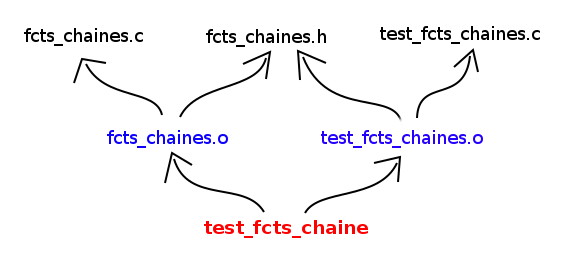
\includegraphics[scale=0.5]{graphe_dep.png}
%  \end{center}
%
%\item La fonction min\_2\_maj supplémentaire n'implique pas d'ajout
%  de fichier ni modification des dépendances des fichiers. Il n'y a
%  donc pas besoin de changer le Makefile pour la prendre en compte.
%
%\newpage
%
%\item Les fonctions \texttt{mon\_strcmp} et \texttt{min\_2\_maj}
%  prennent en arguments deux pointeurs vers des tableaux de
%  \texttt{char}.
%
%  Considérons le bout de code suivant :
%
%  \begin{lstlisting}
%    int mon_strcmp(char s1[], char s2[]) {
%      [...]
%    }
%
%    int main(int argc, char * argv[]) {
%      char chaine1[10] = "abcdefghi";
%      char chaine2[10] = "jklmnopqr";
%
%      mon_strcmp(chaine1, chaine2);
%    }
%  \end{lstlisting}
%
%  En langage C, le passage des paramètres se fait \textbf{par copie}. \\
%
%  On pourrait donc penser que lors de l'appel de \texttt{mon\_strcmp}, tout le
%  contenu des deux
%  tableaux de caractères \texttt{chaine1} et \texttt{chaine2} serait copié dans
%  les nouvelles variables \texttt{s1} et \texttt{s2}. \textbf{Ce n'est pas le cas !}
%  En effet, les paramètres de la fonction sont de type \texttt{char[]}
%  (équivalent à \texttt{char*}) et sont
%  donc des pointeurs. On a vu en TD que lorsqu'on déclare par exemple :
%
%\begin{verbatim}
%  int tab[10];
%\end{verbatim}
%
%  on obtient dans la variable \texttt{tab} un pointeur
%  contenant l'adresse de la première case du tableau. \\
%
%  Ainsi, lorsqu'on appelle \texttt{mon\_strcmp} avec comme
%  arguments chaine1 et chaine2, ce ne sont pas les tableaux entiers qui sont
%  copiés mais simprement les variables contenant leurs adresses.
%
%\item Taille du type \texttt{unsigned char} : \textbf{1} octet, c'est à dire
%  \textbf{8} bits \\
%  Taille maximale d'un entier représenté avec un \texttt{unsigned char} :
%  \textbf{255} \\
%  Intervalle d'entiers tenant sur un \texttt{unsigned char} : de
%  \textbf{0} à \textbf{255}
%
%\item Taille du type \texttt{short int} : \textbf{2} octet, c'est à dire
%  \textbf{16} bits \\
%  Taille maximale d'un entier représenté avec un \texttt{short int} :
%  \textbf{32 767} \\
%  Intervalle d'entiers tenant sur un \texttt{short int} : de
%  \textbf{-32 768} à \textbf{32 767}
%
%\item Le temps d'exécution de \texttt{debordechar} est de l'ordre de la
%  miliseconde. Il n'est donc pas perceptible. Idem pour
%  \texttt{debordeshort}. En revanche, e temps d'exécution de debordeint
%  est d'environs 24 secondes selon l'ordinateur sur lequel le programme est
%  exécuté.
%
%  On peut mesurer le temps d'exécution d'une commande shell à l'aide de la
%  commande \texttt{time}. Ainsi :
%
%\begin{verbatim}
%user@computer$ time ./debordechar
%
%real    0m0.002s
%user    0m0.000s
%sys     0m0.000s
%\end{verbatim}
%
%La taille d'un \texttt{long} (8 octets) est plus grande que celle d'un
%\texttt{int} d'un facteur $$ 2^{64} / 2^{32} $$ soit  environs 4 milliards. Il
%n'est donc pas possible de mesurer le temps d'exécution de \texttt{debordelong}
%car le DLST ferme la nuit.
%
%\newpage
%
%\item Conversion d'une chaine de caractères en entier selon l'algorithme de
%  Horner :
%
%  \lstinputlisting{listing/horner.c}
%
%\item Le script \texttt{make\_gen.sh} se décompose en plusieurs blocs :
%  \begin{description}
%
%  \item [Bloc 1] Comme vu en TP3, le bloc 1 déclare une fonction qui prend un
%    nom de fichier en argument,
%    en extrait à l'aide de la commande \texttt{grep} toutes les lignes contenant
%    ``\#include'', puis extrait de chaque ligne le nom du fichier inclu à l'aide
%    de la commande \texttt{sed}. La liste de tous les fichiers obtenus séparés
%    par des espaces est
%    ensuite imprimée sur la sortie standard.
%
%  \item [Bloc 2] Le bloc 2 renvoie une erreur si le script n'a pas été appelé
%    avec un unique argument. Un message d'erreur indique que cet argument doit
%    être le nom de l'exécutable que l'on souhaite obtenir.
%
%  \item [Bloc 3] Le bloc 3 déclare la variable PRGM qui contient le premier
%    argument passé au script, soit le nom du programme qu'on souhaite obtenir.
%
%  \item [Bloc 4] Le bloc 4 effectue les actions suivantes :
%    \begin{itemize}
%    \item Il déclare la variable \texttt{DEPPRGM} qui
%      contient une cible de Makefile pour fabriquer le programme principal que
%      l'utilisateur a donné en premier argument du script.
%
%    \item Il déclare la variable \texttt{COMPRGM} qui contient la commande
%      Makefile à exécuter pour la
%      cible contenue dans \texttt{DEPPRGM}, la ligne commançant bien par une
%      tabulation (``\verb|\t|'') et pas par des espaces.
%
%    \item Ensuite, pour chaque fichier se terminant par \texttt{.c}, le nom du
%      fichier
%      sans son extension est obtenu à l'aide de la commande \texttt{basename} et
%      on y ajoute ensuite l'extension \texttt{.o}. On obtient ainsi le fichier
%      objet que l'on souhaite construire pour satisfaire les dépendances du
%      programme principal.
%
%    \item Ces fichiers objet sont ensuite ajoutés à la fin des deux variables
%      \texttt{DEPPRGM} et \texttt{COMPRGM}.
%
%    \item Enfin, la cible ainsi construite et sa commande sont ajouté dans un
%      fichier
%      Makefile qui est écrasé s'il existait déjà.
%    \end{itemize}
%
%  \item [Bloc 5] Le dernier bloc ajoute au Makefile les cibles pour construire
%    tous les fichiers objet dont le programme principal va dépendre.
%
%  \end{description}
%
%\newpage
%
%\item Script \texttt{make\_gen.sh} complété :
%
%  \lstinputlisting[style=none]{listing/make_gen.sh}
%







%\vspace*{0.5cm}
%
%
%\columnratio{0.8,0.2}
%\begin{paracol}{2}
%  \begin{leftcolumn}
%    \begin{enumerate}
%      \setcounter{enumi}{1}
%    \item Edgar se place dans son répertoire personnel et lance la commande :
%\begin{verbatim}
%        cp ../dude/../dude/tp2 ~/./révision/tp2
%\end{verbatim}
%Sa commande va-t-elle fonctionner ? Comment aurait-il pu la simplifier ?
%    \end{enumerate}
%  \end{leftcolumn}
%
%\begin{rightcolumn}
%  \dirtree{%
%    .1 /.
%    .2 home.
%    .3 dude.
%    .4 tp2.
%    .3 edgar.
%    .4 révision.
%  }
%\end{rightcolumn}
%\end{paracol}
%
%\vspace{2cm}
%
%\begin{enumerate}
%  \setcounter{enumi}{2}
%\item On souhaite écrire un script qui indique l'appartenance d'un entier à un intervalle. Par exemple, on doit pouvoir vérifier que 4 est compris entre 3 et 10 en tapant :
%\begin{verbatim}
%  ./intervalle.sh 3 10 4
%\end{verbatim}
%\begin{enumerate}
%\item Écrire le test (le if) pour vérifier que l'utilisateur a bien donné 3 arguments
%
%  \vspace{2cm}
%
%\item Écrire le bout de code qui affiche {\tt OK} si le 3\textsuperscript{ème} argument est bien compris entre le 1\textsuperscript{er} et le 2\textsuperscript{ème}, et {\tt KO} sinon
%\end{enumerate}
%
%\newpage
%
%\item Écrire un script qui liste tous les fichiers finissant par {\tt .sh} et qui leur donne le droit d'exécution si :
%  \begin{itemize}
%  \item Le fichier n'est pas déjà exécutable
%  \item Le fichier n'est pas un répertoire
%  \item Le fichier n'est pas vide
%  \end{itemize}
%
%\vspace{8cm}
%
%\item Edgar (encore lui) souhaite avoir un programme qui affiche un compte à rebours (10, 9, 8 ...). Pour ce faire, il écrit le script suivant :
%
%  \vspace{0.2cm}
%
%\begin{verbatim}
%1       #!/bin/bash
%2       decompte() {
%3           if [ $1 -eq 0 ]      # Si on arrive à 0, on s'arrête
%4           then
%5               exit 0
%6           fi
%7           echo $1              # On dit où on en est
%8           suiv=$(expr $1 - 1)  # On calcule le chiffre suivant
%9           decompte $suiv       # On appelle la fonction avec le chiffre suivant
%10      }
%11
%12      decompte 10              # On lance un décompte à partir de 10
%\end{verbatim}
%
%  \vspace{0.2cm}
%
%\begin{enumerate}
%\item Est-ce que son script va fonctionner ?
%
%  \vspace{2cm}
%
%\item Si, à la ligne 9, Edgar avait appelé : {\tt decompte \$1} au lieu de : {\tt decompte \$suiv}, que se serait-il passé ?
%\end{enumerate}
%
%
%\end{enumerate}
%
%\vspace{2cm}
%
\end{document}
